\documentclass[a4paper,12pt]{article}
\usepackage{latexsym}
\usepackage{graphicx}
\usepackage{epsfig}
\usepackage{float}
\usepackage{natbib}
\graphicspath{{./}}
\DeclareGraphicsExtensions{.eps}
\author{Howard Kinsman}
\title{Computational Astrophysics Project 1 - Investigation of Lutz-Kelker bias, through Monte Carlo simulations, on estimation of stellar distance using trigonometric parallax}
\begin{document}
\maketitle
\begin{abstract}
Monte Carlo simulations were carried out with a randomly generated sample of 400,000 stars and derived absolute magnitudes and distances were retrieved from the sample with assumed parallax and photometric errors. The resulting derived data were compared with the 'true' data and the error dispersion was found to be consistent with the well known Lutz-Kelker bias.
\end{abstract}
{\bf Keywords:} Lutz-Kelker bias, Monte Carlo simulation, stars: distances, magnitude, parallax

\section{Introduction}
The Lutz-Kelker bias was first quantified \citep{lutz} using the absolute magnitude of stars estimated with trigonometric parallax. It occurs because the number of observable stars increases with the square of the distance. For any given parallax measurement there will be an error which will give an upper and lower bound of retrieved distance, and stars at a smaller distance and stars further away can scatter into this volume, however as there are more stars outside the sampled volume than inside, the sample will be biased. This effect causes a systematic bias such that measured parallaxes will on average yield too small distances \citep{oud}. Monte Carlo simulations are ideally placed to investigate this phenomenom and provide corrections and the necessary calibration to trigonometric parallax measurements.
\newpage
\section{Monte Carlo simulations}
Four Monte Carlo simulations were carried out, each with a sample of 400,000 stars having a true absolute magnitude of 0.6 (with a Gaussian dispersion of 0.001 mag.). The stars were assigned true distances of between 1pc and 8Kpc. A small $\sigma$ photometric error of 0.01 mag. in the measurement of the retrieved absolute magnitude was assumed in each case. Please note that the original LKbiasMSc.f program had a small bug associated with photometric error - this was corrected prior to running these simulations. Only stars within a retrieved distance of 4Kpc were considered.

\subsection{Task 1}
For this simulation a constant spatial density distribution of stars was assumed. This simulation employed a constant parallax error of 50 microarcsec. There was no apparent magnitude limit. The total mean and standard deviation of the retrieved absolute magnitudes are shown in Table \ref{tab:task1} together with the mean and standard deviations after the results were split into 1000pc bins. This is shown graphically in Figures \ref{fig:t1bin1} to \ref{fig:t1bin4}. A scatter plot of retrieved absolute magnitude as a function of retrieved distance is shown in Figure \ref{fig:t1graph1}. Figures \ref{fig:t1graph2} and \ref{fig:t1graph3} show the number distribution of stars for true and retrieved distance respectively.

\begin{table}[ht]
\centering
\begin{tabular}{|l|l|l|}
\hline
Distance (pc) & Mean & Std Deviation \\
\hline
Total & 1.0355 & 0.4797 \\
0-1000 & 0.6122 & 0.1055 \\
1001-2000 & 0.6945 & 0.2049 \\
2001-3000 & 0.8561 & 0.3629 \\
3001-4000 & 1.1057 & 0.4977 \\
\hline
\end{tabular}
\caption{\label{tab:task1}Mean retrieved absolute magnitudes (Task 1)}
\end{table}

\begin{figure}[H]
\centering
\includegraphics[width=0.75\textwidth]{./Task1/Bin1}
\caption{Task 1 -  Distribution of Retrieved Abs. Mag. (0-1000 pc)}
\label{fig:t1bin1}
\end{figure}

\begin{figure}[H]
\centering
\includegraphics[width=0.75\textwidth]{./Task1/Bin2}
\caption{Task 1 - Distribution of Retrieved Abs. Mag. (1001-2000 pc)}
\label{fig:t1bin2}
\end{figure}

\begin{figure}[H]
\centering
\includegraphics[width=0.75\textwidth]{./Task1/Bin3}
\caption{Task 1 - Distribution of Retrieved Abs. Mag. (2001-3000 pc)}
\label{fig:t1bin3}
\end{figure}

\begin{figure}[H]
\centering
\includegraphics[width=0.75\textwidth]{./Task1/Bin4}
\caption{Task 1 - Distribution of Retrieved Abs. Mag. (3001-4000 pc)}
\label{fig:t1bin4}
\end{figure}

\begin{figure}[H]
\centering
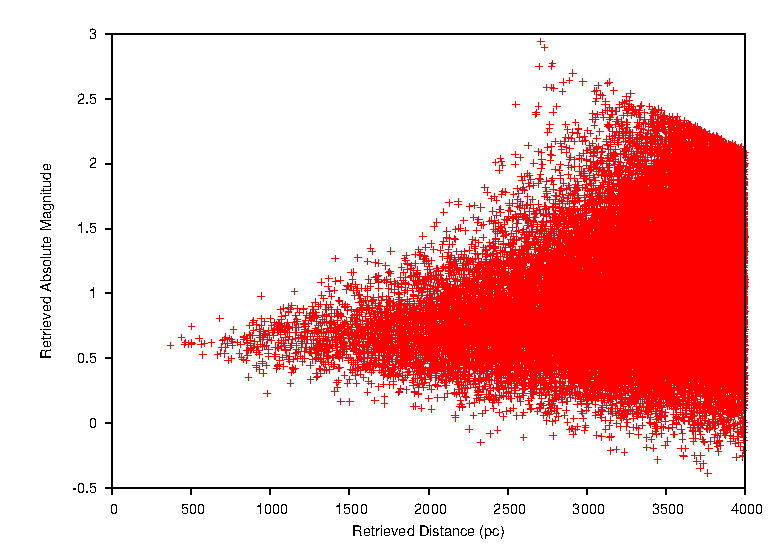
\includegraphics[width=0.75\textwidth]{./Task1/Graph1}
\caption{Task 1 - Retrived Absolute Magntude as a function of Retrieved Distance}
\label{fig:t1graph1}
\end{figure}

\begin{figure}[H]
\centering
\includegraphics[width=0.75\textwidth]{./Task1/Graph2}
\caption{Task 1 - Number distribution of stars by True Distance}
\label{fig:t1graph2}
\end{figure}

\begin{figure}[H]
\centering
\includegraphics[width=0.75\textwidth]{./Task1/Graph3}
\caption{Task 1 - Number distribution of stars by Retrieved Distance}
\label{fig:t1graph3}
\end{figure}
\newpage
\subsection{Task 2}
This simulation used the same parameters as Task 1 except an apparent magnitude limit of 14 was assumed. Table \ref{tab:task2} and figures \ref{fig:t2bin1} to \ref{fig:t2graph3} are the same plots as used for Task 1.
 
\begin{table}[ht]
\centering
\begin{tabular}{|l|l|l|}
\hline
Distance (pc) & Mean & Std Deviation \\
\hline
Total & 0.7992 & 0.3082 \\
0-1000 & 0.6069 & 0.1182 \\
1001-2000 & 0.6915 & 0.1963 \\
2001-3000 & 0.8363 & 0.3252 \\
3001-4000 & 0.7929 & 0.3061 \\
\hline
\end{tabular}
\caption{\label{tab:task2}Mean retrieved absolute magnitudes (Task 2)}
\end{table}

\begin{figure}[H]
\centering
\includegraphics[width=0.75\textwidth]{./Task2/Bin1}
\caption{Task 2 -  Distribution of Retrieved Abs. Mag. (0-1000 pc)}
\label{fig:t2bin1}
\end{figure}

\begin{figure}[H]
\centering
\includegraphics[width=0.75\textwidth]{./Task2/Bin2}
\caption{Task 2 - Distribution of Retrieved Abs. Mag. (1001-2000 pc)}
\label{fig:t2bin2}
\end{figure}

\begin{figure}[H]
\centering
\includegraphics[width=0.75\textwidth]{./Task2/Bin3}
\caption{Task 2 - Distribution of Retrieved Abs. Mag. (2001-3000 pc)}
\label{fig:t2bin3}
\end{figure}

\begin{figure}[H]
\centering
\includegraphics[width=0.75\textwidth]{./Task2/Bin4}
\caption{Task 2 - Distribution of Retrieved Abs. Mag. (3001-4000 pc)}
\label{fig:t2bin4}
\end{figure}

\begin{figure}[H]
\centering
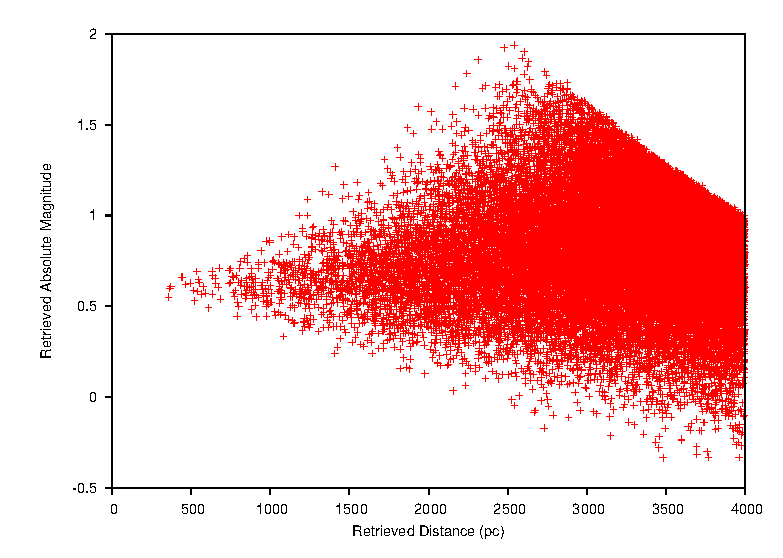
\includegraphics[width=0.75\textwidth]{./Task2/Graph1}
\caption{Task 2 - Retrived Absolute Magntude as a function of Retrieved Distance}
\label{fig:t2graph1}
\end{figure}

\begin{figure}[H]
\centering
\includegraphics[width=0.75\textwidth]{./Task2/Graph2}
\caption{Task 2 - Number distribution of stars by True Distance}
\label{fig:t2graph2}
\end{figure}

\begin{figure}[H]
\centering
\includegraphics[width=0.75\textwidth]{./Task2/Graph3}
\caption{Task 2 - Number distribution of stars by Retrieved Distance}
\label{fig:t2graph3}
\end{figure}

\newpage
\subsection{Task 3}
This simulation used the same parameters as Task 1 except the spatial density of stars was no longer assumed to be constant but decreasing as $R^{-2}$ where R is the distance between 1pc and 8Kpc. Table \ref{tab:task3} and figures \ref{fig:t3bin1} to \ref{fig:t3graph3} are the same plots as used for Task 1.
 
\begin{table}[ht]
\centering
\begin{tabular}{|l|l|l|}
\hline
Distance (pc) & Mean & Std Deviation \\
\hline
Total & 0.7859 & 0.3785 \\
0-1000 & 0.6095 & 0.0792 \\
1001-2000 & 0.6528 & 0.1822 \\
2001-3000 & 0.7404 & 0.3158 \\
3001-4000 & 0.8842 & 0.4541 \\
\hline
\end{tabular}
\caption{\label{tab:task3}Mean retrieved absolute magnitudes (Task 3)}
\end{table}

\begin{figure}[H]
\centering
\includegraphics[width=0.75\textwidth]{./Task3/Bin1}
\caption{Task 3 -  Distribution of Retrieved Abs. Mag. (0-1000 pc)}
\label{fig:t3bin1}
\end{figure}

\begin{figure}[H]
\centering
\includegraphics[width=0.75\textwidth]{./Task3/Bin2}
\caption{Task 3 - Distribution of Retrieved Abs. Mag. (1001-2000 pc)}
\label{fig:t3bin2}
\end{figure}

\begin{figure}[H]
\centering
\includegraphics[width=0.75\textwidth]{./Task3/Bin3}
\caption{Task 3 - Distribution of Retrieved Abs. Mag. (2001-3000 pc)}
\label{fig:t3bin3}
\end{figure}

\begin{figure}[H]
\centering
\includegraphics[width=0.75\textwidth]{./Task3/Bin4}
\caption{Task 3 - Distribution of Retrieved Abs. Mag. (3001-4000 pc)}
\label{fig:t3bin4}
\end{figure}

\begin{figure}[H]
\centering
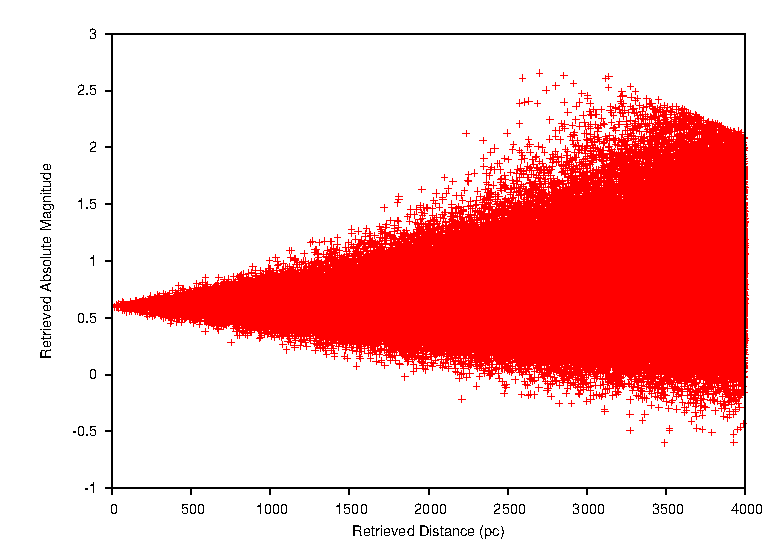
\includegraphics[width=0.75\textwidth]{./Task3/Graph1}
\caption{Task 3 - Retrived Absolute Magntude as a function of Retrieved Distance}
\label{fig:t3graph1}
\end{figure}

\begin{figure}[H]
\centering
\includegraphics[width=0.75\textwidth]{./Task3/Graph2}
\caption{Task 3 - Number distribution of stars by True Distance}
\label{fig:t3graph2}
\end{figure}

\begin{figure}[H]
\centering
\includegraphics[width=0.75\textwidth]{./Task3/Graph3}
\caption{Task 3 - Number distribution of stars by Retrieved Distance}
\label{fig:t3graph3}
\end{figure}

\newpage
\subsection{Task 4}
This simulation used the same parameters as Task 2 (an apparent magnitude limit of 14) except the parallax error was no longer assumed to be constant but had a GAIA-like error distribution. Table \ref{tab:task4} and figures \ref{fig:t4bin1} to \ref{fig:t4graph3} are the same plots as used for Task 1.
 
\begin{table}[ht]
\centering
\begin{tabular}{|l|l|l|}
\hline
Distance (pc) & Mean & Std Deviation \\
\hline
Total & 0.6286 & 0.0944 \\
0-1000 & 0.5866 & 0.0834 \\
1001-2000 & 0.6017 & 0.0239 \\
2001-3000 & 0.61 & 0.0554 \\
3001-4000 & 0.6376 & 0.1067 \\
\hline
\end{tabular}
\caption{\label{tab:task4}Mean retrieved absolute magnitudes (Task 4)}
\end{table}

\begin{figure}[H]
\centering
\includegraphics[width=0.75\textwidth]{./Task4/Bin1}
\caption{Task 4 -  Distribution of Retrieved Abs. Mag. (0-1000 pc)}
\label{fig:t4bin1}
\end{figure}

\begin{figure}[H]
\centering
\includegraphics[width=0.75\textwidth]{./Task4/Bin2}
\caption{Task 4 - Distribution of Retrieved Abs. Mag. (1001-2000 pc)}
\label{fig:t4bin2}
\end{figure}

\begin{figure}[H]
\centering
\includegraphics[width=0.75\textwidth]{./Task4/Bin3}
\caption{Task 4 - Distribution of Retrieved Abs. Mag. (2001-3000 pc)}
\label{fig:t4bin3}
\end{figure}

\begin{figure}[H]
\centering
\includegraphics[width=0.75\textwidth]{./Task4/Bin4}
\caption{Task 4 - Distribution of Retrieved Abs. Mag. (3001-4000 pc)}
\label{fig:t4bin4}
\end{figure}

\begin{figure}[H]
\centering
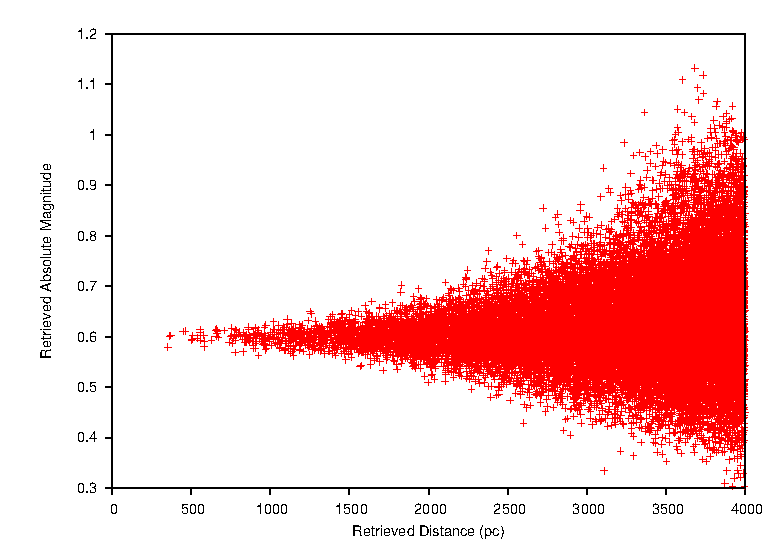
\includegraphics[width=0.75\textwidth]{./Task4/Graph1}
\caption{Task 4 - Retrived Absolute Magntude as a function of Retrieved Distance}
\label{fig:t4graph1}
\end{figure}

\begin{figure}[H]
\centering
\includegraphics[width=0.75\textwidth]{./Task4/Graph2}
\caption{Task 4 - Number distribution of stars by True Distance}
\label{fig:t4graph2}
\end{figure}

\begin{figure}[H]
\centering
\includegraphics[width=0.75\textwidth]{./Task4/Graph3}
\caption{Task 4 - Number distribution of stars by Retrieved Distance}
\label{fig:t4graph3}
\end{figure}

\newpage
\section{Discussion}
The mean of the total sample, 1.0355 as shown in Table \ref{tab:task1}, has clearly diverged from the true mean absolute magnitude of 0.6. With a dispersion (standard deviation) of 0.4797 it is not a true representive of the sample: there is a bias. Table \ref{tab:task1} and Figures \ref{fig:t1bin1} to \ref{fig:t1bin4} from the Task 1 simulation show that the margin of error in retrieved absolute magnitude grows with the retrieved distance. Stars within 2Kpc are showing a mean absolute magnitude that is approximately 0.6 but for more distant stars the standard deviation grows sharply with distance. The scatter plot in Figure \ref{fig:t1graph1} illustrates this further with a strong tendency towards larger (less bright) absolute magnitudes with greater distance.

Figures \ref{fig:t1graph2} and \ref{fig:t1graph3} help explain the above error margin by showing that the number distribution of stars selected by retrieved distance is far greater than those selected by true distance. This is consistent with the Lutz-Kelker bias: the retrieved distances are seen to be smaller than they acually are, causing a greater number of more distant stars to be pulled into the sample than nearby stars, creating a bias.

In addition to the Lutz-Kelker bias another form of bias needs to be taken into account and that is caused by error propogation. In this case as $R=1/p$ (R=distance, p=parallax) there is an inverse relationship between the measurement (parallax) and the derived quantity (distance) which leads to an asymmetric error i.e. the error will become greater the more distant the star.

In Task 2 an apparent magnitude limit of 14 was assumed. This simulation resulted in a much improved total mean absolute magnitude and lower error dispersions in the various bins in Table \ref{tab:task2} and Figures \ref{fig:t2bin1} to \ref{fig:t2bin4}. This can be attributed to the number distribution of stars sampled for true and retrieved distances, as can be seen in Figures \ref{fig:t2graph2} and \ref{fig:t2graph3} the number of stars in both figures are similar. Lutz determined that in a magnitude limited sample the Lutz-Kelker corrections should not be applied \citep{lutz2}. There is however a bias still associated with a magnitude limited sample: the Malmquist bias, which is the preferential selection of intrinsically bright objects.

Task 3 assumed a stellar spatial density decreasing by $R^{-2}$ whereas the previous simulations all assumed a constant spatial density. The results, Table \ref{tab:task3} and Figures \ref{fig:t3bin1} to \ref{fig:t3graph3} again show a reduction in the error. So it seems that an exponentially declining spatial stellar density does go some way to counteract the Lutz-Kelker bias. The Milky Way is disk shaped so is clearly not uniform in structure and some Kutz-Kelker calibrations do attempt to take scale height, direction and large scale structure into account \citep{smith}. There is an exponential decrease of projected density with galactocentric radius for spiral galaxies \citep{smith}.

Finally, Task 4 introduced a Gaia-like error approximation, together with the apparent magnitude limit of 14 from Task 2. This simulation produced results with very low margins of error, see Table \ref{tab:task4} and Figures \ref{fig:t4bin1} to \ref{fig:t4graph3}, even at large distances. Lutz-Kelker corrections and calibration therefore can, and should, be taken into account when estimating distance with trigonometric parallax. However, as can be seen from the Gaia-like error corrections, these calibrations themselves also need revision as technological improvements increase the accuracy of parallax measurements.

\begin{thebibliography}{1}
\bibitem[Lutz(1983)]{lutz2}Lutz, T.E., Nearby Stars and the Stellar Luminosity Function, 1983, IAU Coll, 76
\bibitem[Lutz and Kelker(1973)]{lutz}Lutz, T.E., Kelker, D.H., On the use of Trigonometric Parallaxes for the Calibration of Luminosity Systems: Theory, 1973, Publications of the Astronomical Society of the Pacific, 85, 573
\bibitem[Oudmaijer et al.(1997)]{oud}Oudmaijer. R.D., Groenewegen, M.A.T., Schrijver, H., The Lutz-Kelker bias in trigonometric parallaxes, 1997, Monthly Notices of the Royal Astronomical Society, 294, 41-46 
\bibitem[Smith(1999)]{smith}Smith, H., The Lutz-Kelker effect in the Hipparcus era and beyond, 1998, Modern Astrometry and Astrodynamics, 1999
\end{thebibliography}
\end{document}
